\documentclass[12pt]{article}
\usepackage[utf8]{inputenc}
\usepackage[a4paper, total={6in, 8in}, margin=1in]{geometry}
\usepackage{titlesec}
\usepackage[backend=biber, style=ieee]{biblatex}
\usepackage{graphicx}
\usepackage{amsmath}
\usepackage{amssymb}
\usepackage{amstext}
\usepackage{array}
\usepackage{xcolor}
\usepackage{multicol}


\newcolumntype{L}{>{$}1<{$}}  % Math mode table

\addbibresource{main.bib}

\newcolumntype{L}{>{$}l<{$}}  % Math mode table
\newcolumntype{R}{>{$}r<{$}}  % Math mode table
\newcolumntype{C}{>{$}c<{$}}  % Math mode table

\titleformat{\section}
  {\normalfont\fontsize{14}{15}\bfseries}{\thesection}{1em}{}

\titleformat{\subsection}
  {\normalfont\fontsize{12}{15}\bfseries}{\thesubsection}{1em}{}

\title{AES 670 Midterm}
 \author{Mitchell Dodson}
\date{April 11, 2023}

\begin{document}

\maketitle

\section{Surface types}

\begin{figure}[h!]
    \centering
    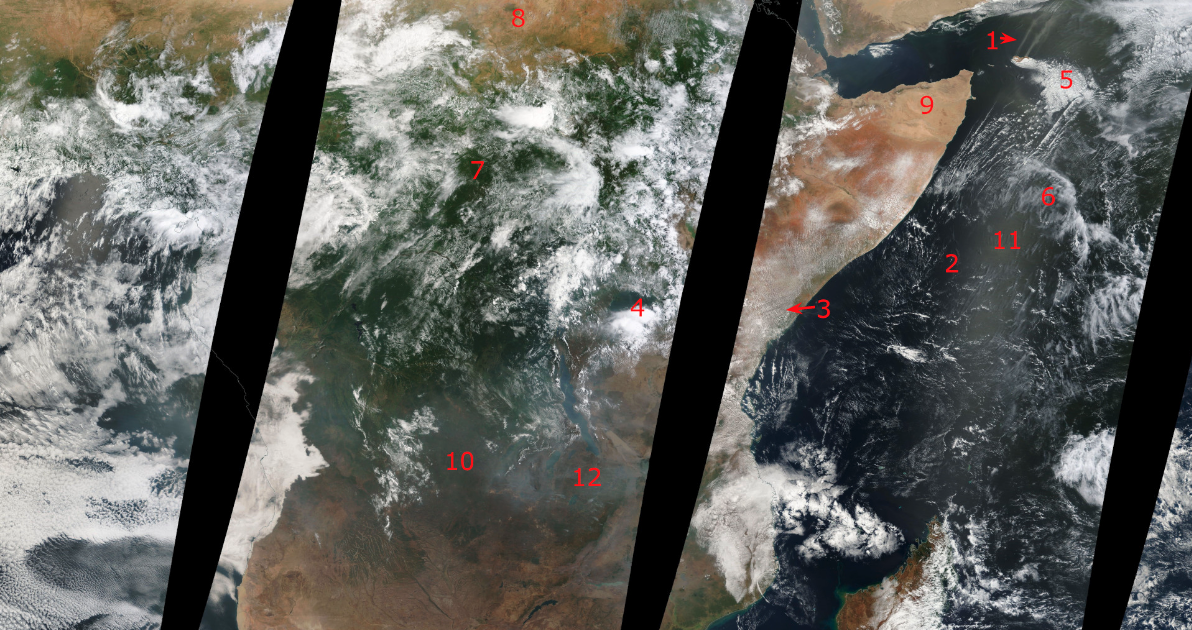
\includegraphics[width=.98\linewidth]{figures/aes670_midterm_numbered.png}

    \caption{Surface types identified in Terra/MODIS atmosphere-corrected reflectance truecolor. Captured September 5, 2022.}
    \label{q1_numbered}
\end{figure}

\begin{multicols}{2}
\begin{enumerate}
    \item{Smoke or dust plumes}
    \item{Sea surface}
    \item{Cumulus streets}
    \item{Towering mesoscale convective system}
    \item{Stratocumulus shield}
    \item{High cirrus clouds}
    \item{Rainforest}
    \item{Savannah/steppe}
    \item{Arid/barren desert}
    \item{Temperate forest}
    \item{Sun glint on water surface}
    \item{Smoke plumes}
\end{enumerate}
\end{multicols}

\clearpage

\section{Data voids}

The black stripes found in multi-swath composites of MODIS imagery are the consequence of the divergence of the polar-orbiting satellites' orbit tracks over the equator due to Earth's roughly spherical shape. Terra and Aqua orbit at a rate of 14 revolutions per day, and achieve global coverage with the exception of these dead zones every 24 hours.

In order to get rid of the stripes while maintaining daily global coverage, the radiometers would either need to have wider FOVs, or the satellites would need to complete a greater number of orbits per day with less zonal precession per orbit. An additional problem with the latter option is that the satellites would no longer be sun-synchronous unless the altitude was decreased (angular speed increased) to account for the new orbits, which would exacerbate the FOV problem. Nonetheless it is theoretically possible, if impractical, to avoid the stripes with changes to the instrument or orbit.

\section{Surface temperature bands}

Using a naive approach to estimate land surface temperature with only one band, I would choose a clean longwave window band in the $10.3\mu m - 11.4\mu m$ range, which is less affected by water vapor, ozone, and carbon dioxide absorption than other thermal bands. The land surface temperature may be estimated by scaling the observed radiance by the approximate emissivity of the surface, then inverting Planck's function with the radiance to retrieve an approximate temperature.

The aforementioned method doesn't take into account artificial cooling dominantly caused by variation in precipitable water vapor in the atmospheric column, so an improved method of estimating land surface temperature involves a linear combination of radiance from a "clean" thermal band like $10.3\mu m$ and a "dirty" thermal band like $12.3\mu m$, which is derived from a radiative transfer model for a clear-sky pixel. The difference between the two bands correlates with the precipitable water vapor, which is used to estimate and reduce the bias on actual land surface temperature.

\clearpage

\section{RGB composites of region}

\begin{figure}[h!]
    \centering
    %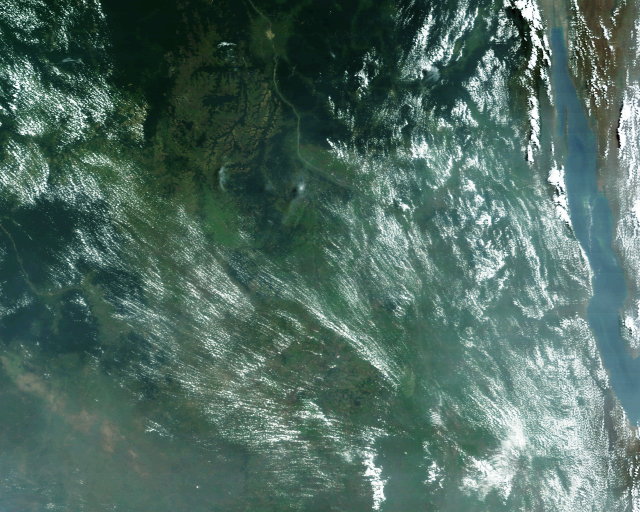
\includegraphics[width=.62\linewidth]{figures/rgb_tc.png}

    \begin{center}
        \makebox[\textwidth]{
            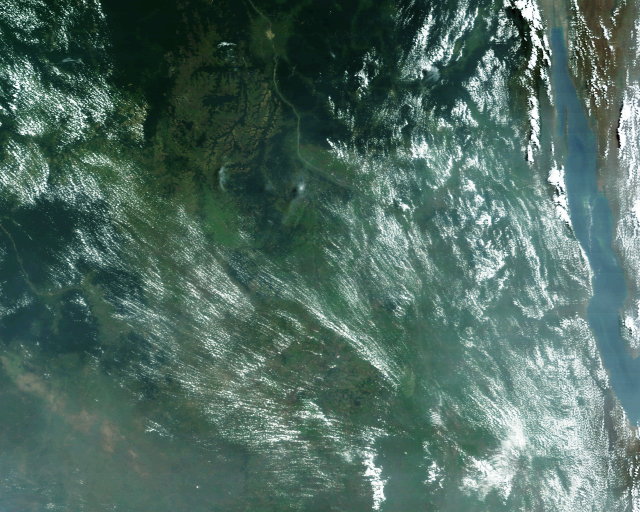
\includegraphics[width=.45\paperwidth]{figures/rgb_tc.png}
            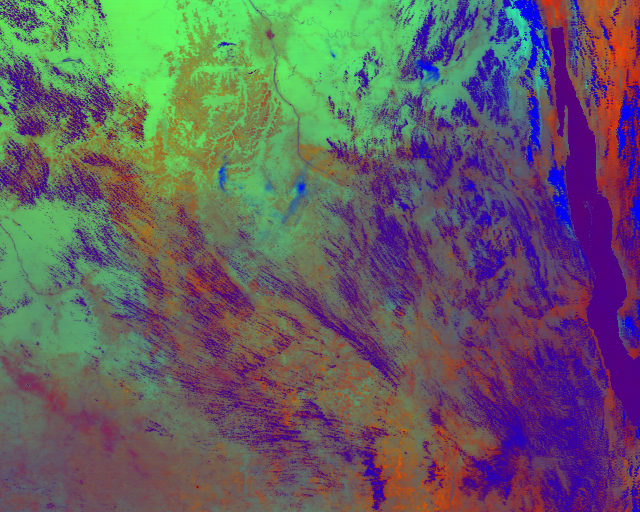
\includegraphics[width=.45\paperwidth]{figures/rgb_custom.png}
        }
    \end{center}

    \begin{center}
        \vspace{-.8em}
        \makebox[\textwidth]{
            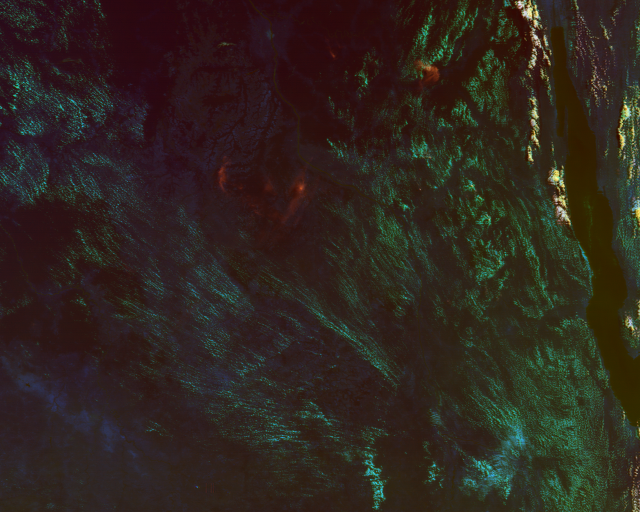
\includegraphics[width=.3\paperwidth]{figures/rgb_dcp.png}
            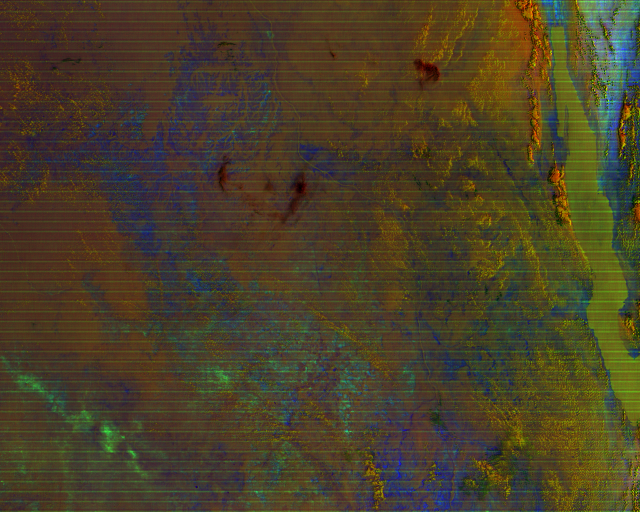
\includegraphics[width=.3\paperwidth]{figures/rgb_dust.png}
            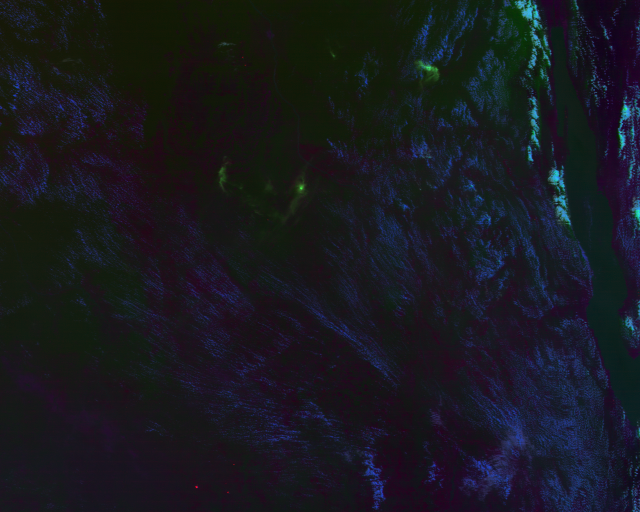
\includegraphics[width=.3\paperwidth]{figures/rgb_fire.png}
        }
    \end{center}

    \caption{Top row: MODIS true-color and custom false-color composites. Bottom row: day cloud-phase (CIMSS recipe), dust, (SPoRT recipe), and custom fire RGBs, all gamma-enhanced to show the appropriate features.}
    \label{q4_rgbs}
\end{figure}

The granule in Figure \ref{q4_rgbs} was captured by Terra on September 5, 2022 at 0835z. The Southern boundary of the Congo rainforest is at the top of the image, and the bottom of the image is a "forest-savanna mosaic" biome.  The Truecolor image shows that the scene is covered by low-level cumulus clouds, and that the lower half of the image is visibly hazier than the top, which I believe is the consequence of smoke from the probable fires shown at the bottom of the fire RGB.

My custom RGB assigns the $11\mu m$ LWIR window channel to RED, NDVI to GREEN, and inverted $8.6\mu m$ LWIR to BLUE. I chose this recipe to distinguish cloud phase and multiple surface emissivities and cloud types (due to the $11-8\mu m$ channel difference), and vegetation amount (with NDVI). The RGB resolves optically thin water and ice clouds, and has good contrast between vegetated and barren land, but doesn't separate low clouds and surface water well.

\clearpage

\section{Surface type reflectances}

\begin{figure}[h!]
    \centering

    \begin{center}
        \makebox[\textwidth]{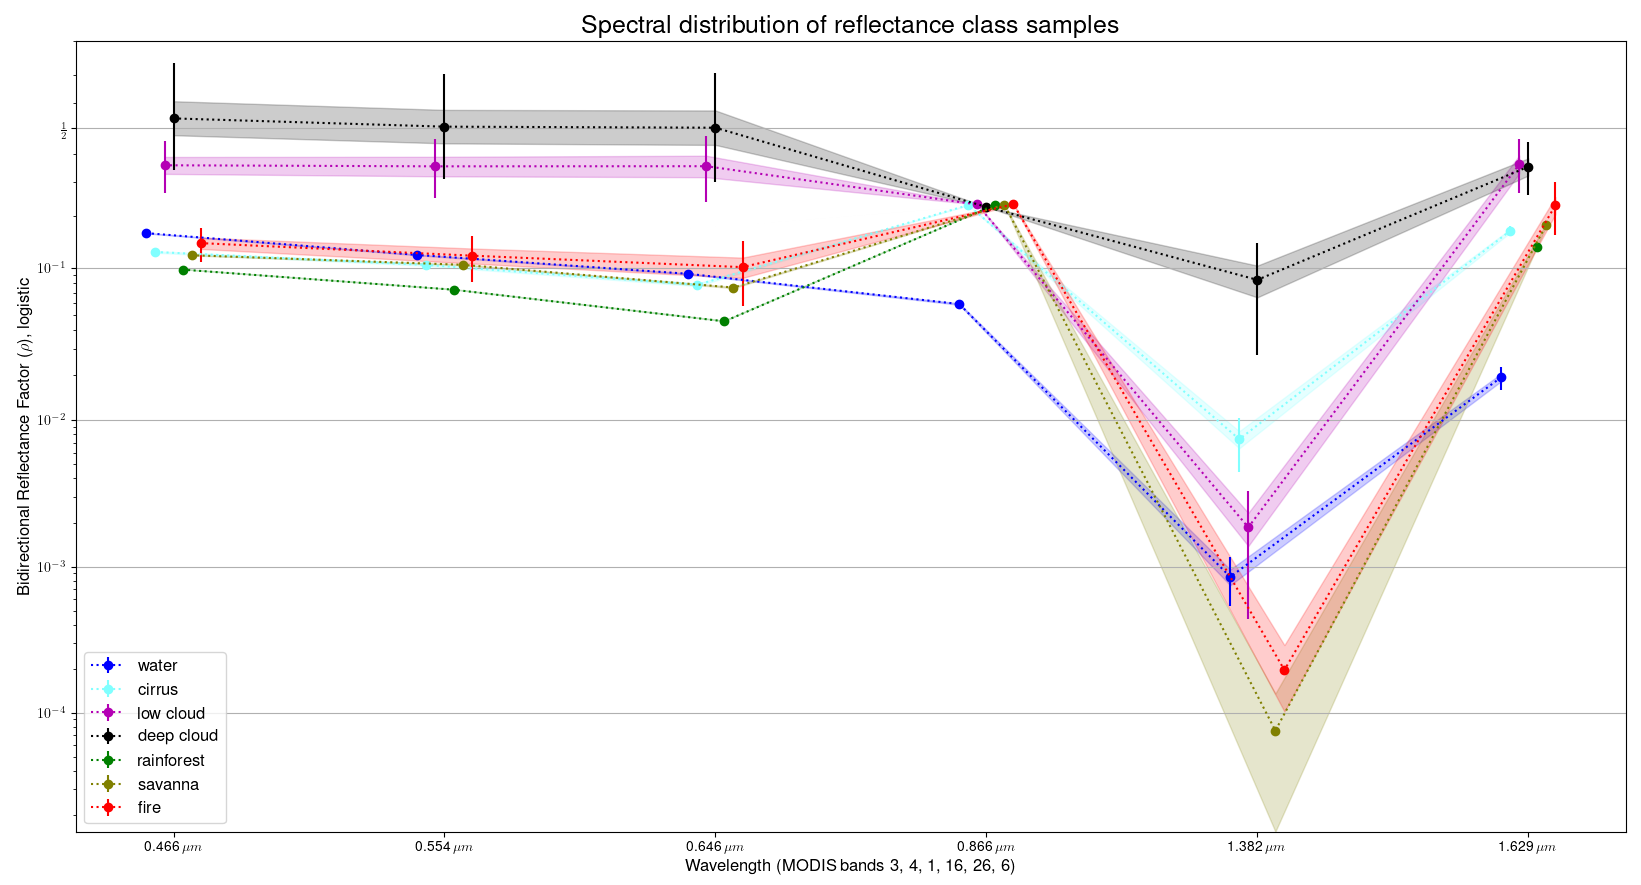
\includegraphics[width=.9\paperwidth]{figures/class_dist_ref_square.png}}
    \end{center}

    \caption{TOA spectral response of pixel samples for 5 surface types in the visible and near-infrared range (logistic scale). As expected, optically-thick clouds are brighter than other classes except for in the $1.382\mu m$ cirrus band, in which water vapor attenuates reflectance from low clouds. Reflectance over water decreases, savanna (soil) reflectance slightly increases, and vegetation reflectance rapidly increases going into the NIR range, which is consistent with the spectral response curves in (Richards, 2022) Figure 3.5.}
    \label{p5_ref_dist}
\end{figure}

\begin{figure}[h!]
    \centering
    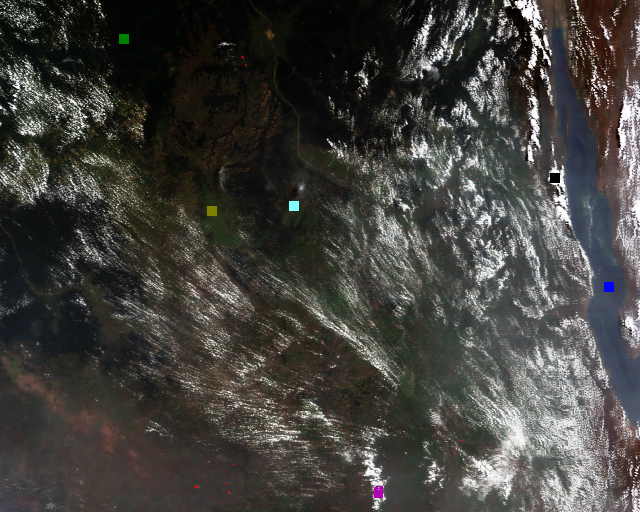
\includegraphics[width=.8\linewidth]{figures/rgb_samples_tc.png}
    
\includegraphics[width=.3\linewidth]{figures/rgb_sample_cbar.png}

    \caption{Location of surface type samples. Left to right, the color bar represents Water, Cirrus, Low Cloud, Deep Cloud, Rainforest, Savanna, and Fire surface types.}
    \label{p5_ref_samples}
\end{figure}

\begin{figure}[h!]
    \centering

    \begin{tabular}{R | C  C | C  C |  C  C }
        & \multicolumn{2}{c|}{0.466 $\mu m$} & \multicolumn{2}{c|}{0.554 $\mu m$} & \multicolumn{2}{c}{0.646 $\mu m$} \\
        \textnormal{Class} &  \mu_1 & \sigma_1 & \mu_2 & \sigma_2 & \mu_3 & \sigma_3 \\
        \hline
        \textnormal{Water} & 0.161 & 0.002  & 0.120 & 0.002  & 0.092 & 0.001  \\
        \textnormal{Cirrus} & 0.125 & 0.004  & 0.104 & 0.004  & 0.078 & 0.004  \\
        \textnormal{Low cloud} & 0.359 & 0.092  & 0.355 & 0.105  & 0.356 & 0.116  \\
        \textnormal{Deep Cloud} & 0.540 & 0.198  & 0.507 & 0.197  & 0.503 & 0.202  \\
        \textnormal{Rainforest} & 0.098 & 0.000  & 0.073 & 0.001  & 0.046 & 0.001  \\
        \textnormal{Savanna} & 0.119 & 0.001  & 0.104 & 0.002  & 0.075 & 0.002  \\
        \textnormal{Fire} & 0.141 & 0.032  & 0.119 & 0.037  & 0.101 & 0.043  \\
    \end{tabular}

    \vspace{1em}

    \begin{tabular}{R | C  C | C  C |  C  C }
        & \multicolumn{2}{c|}{0.866 $\mu m$} & \multicolumn{2}{c|}{1.382 $\mu m$} & \multicolumn{2}{c}{1.629 $\mu m$} \\
        \textnormal{Class} & \mu_4 & \sigma_4 & \mu_5 & \sigma_5 & \mu_6 & \sigma_6 \\
        \hline
        \textnormal{Water} & 0.059 & 0.002  & 0.001 & 0.000  & 0.019 & 0.003 \\
        \textnormal{Cirrus} & 0.230 & 0.000  & 0.007 & 0.003  & 0.166 & 0.012 \\
        \textnormal{Low cloud} & 0.232 & 0.000  & 0.002 & 0.001  & 0.363 & 0.097 \\
        \textnormal{Deep Cloud} & 0.225 & 0.000  & 0.084 & 0.057  & 0.354 & 0.093 \\
        \textnormal{Rainforest} & 0.231 & 0.000  & 0.001 & 0.000  & 0.133 & 0.002 \\
        \textnormal{Savanna} & 0.232 & 0.000  & 0.000 & 0.000  & 0.180 & 0.010 \\
        \textnormal{Fire} & 0.232 & 0.003  & 0.000 & 0.001  & 0.229 & 0.072 \\
    \end{tabular}

    \caption{Means and standard deviations of reflectance-band pixels selected as samples for each surface category.}
    \label{p4_ref_stats}
\end{figure}

\clearpage

\section{Surface type brightness temperatures}

\begin{figure}[h!]
    \centering

    \begin{center}
        \makebox[\textwidth]{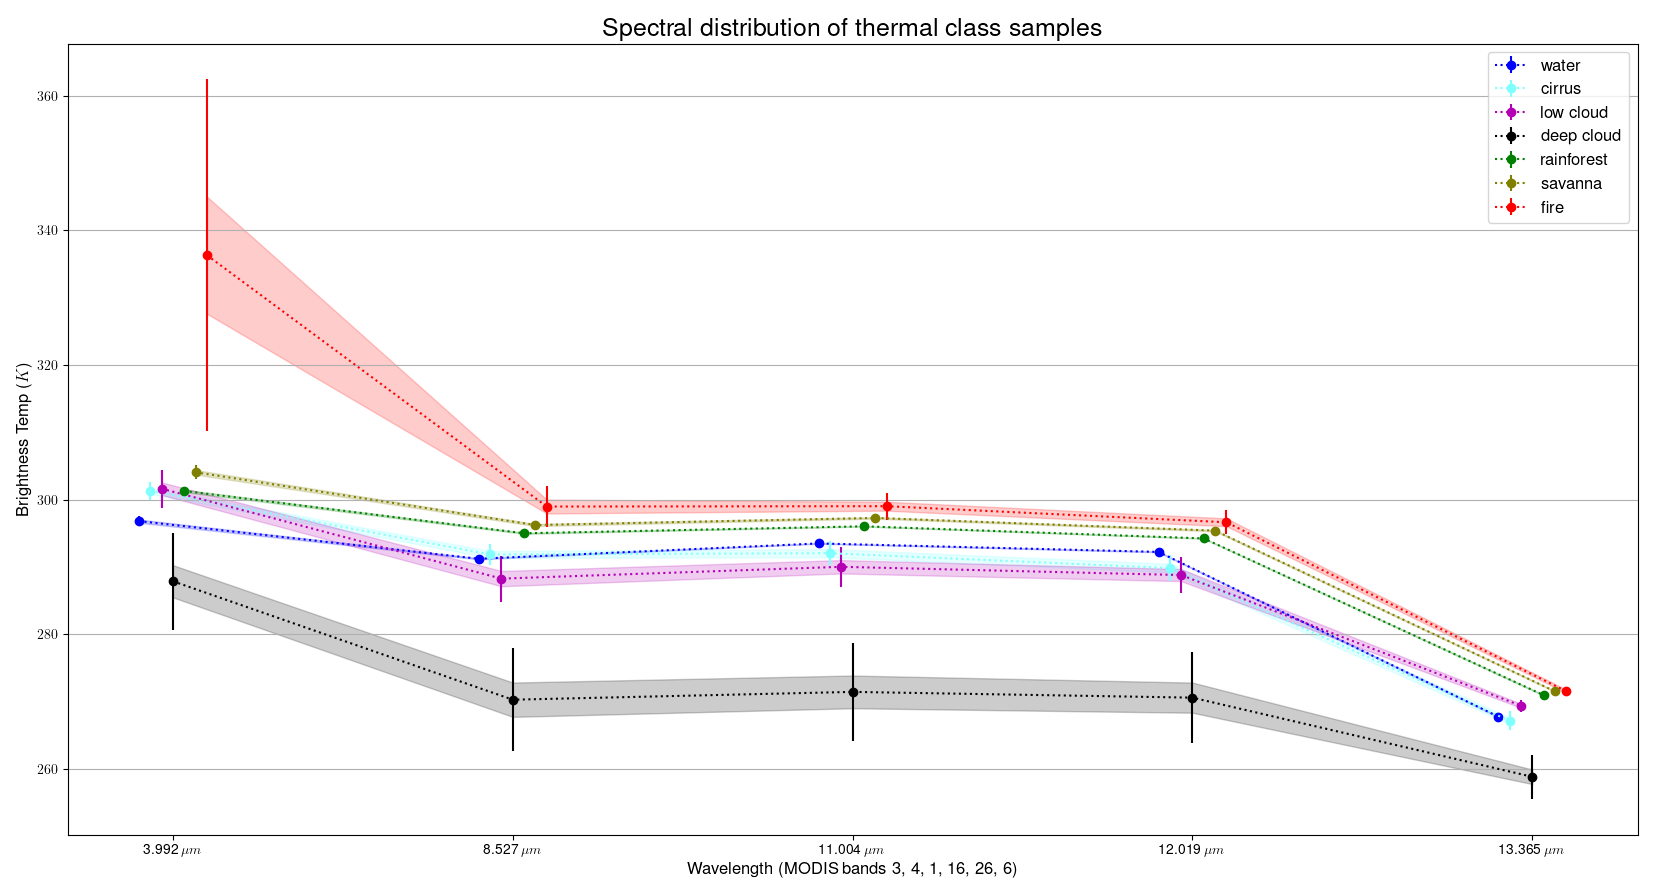
\includegraphics[width=.9\paperwidth]{figures/class_dist_temp_square.png}}
    \end{center}

    \caption{TOA estimated brightness temperatures for each class with $1-\sigma$ error bars. The L1b product I used (MOD021KM) doesn't contain brightness temperature lookup tables for the provided radiance, so I retrieved the temperatures using the inverted Planck function with each band's center wavelength. The fire class is consistently the warmest, especially in the $3.9\mu m$ band, which is close to the peak of the blackbody radiance curve for a typical fire temperature of $600K$. Both land surface types have similar infrared signatures and are consistently warmer than the cloud and water types, except for the rainforest type in the $3.9\mu m$ band which is ``cooler'' than low clouds and cirrus clouds due to the contribution of reflected radiation. Similarly, water appears cooler than low clouds in the $3.9\mu m$ band since liquid surface water strongly absorbs in the NIR range, but the low clouds are reflective. Deep clouds consistently have the lowest brightness temperature since their optical thickness doesn't permit surface emissions and their high cloud-tops are physically cold.}
    \label{p6_temp_dist}
\end{figure}

\begin{figure}[h!]
    \centering

    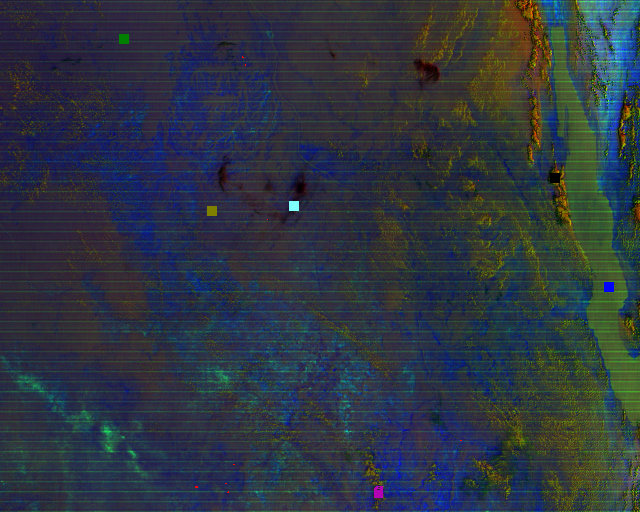
\includegraphics[width=.8\linewidth]{figures/rgb_samples_fc.png}
    
\includegraphics[width=.3\linewidth]{figures/rgb_sample_cbar.png}

    \caption{Location of surface type samples. Left to right, the color bar represents Water, Cirrus, Low Cloud, Deep Cloud, Rainforest, Savanna, and Fire surface types.}
    \label{p6_temp_samples}
\end{figure}

\begin{figure}[h!]
    \centering

    \begin{tabular}{R | C  C | C  C |  C  C }
        & \multicolumn{2}{c|}{3.992 $\mu m$} & \multicolumn{2}{c|}{8.527 $\mu m$} & \multicolumn{2}{c}{11.004 $\mu m$} \\
        \textnormal{Class} & \mu_7 & \sigma_7 & \mu_8 & \sigma_8 & \mu_9 & \sigma_9 \\
        \hline
        \textnormal{Water} & 296.827 & 0.724  & 291.236 & 0.267  & 293.515 & 0.113 \\
        \textnormal{Cirrus} & 301.316 & 1.312  & 291.874 & 1.528  & 292.068 & 1.810  \\
        \textnormal{Low Cloud} & 301.648 & 2.803  & 288.290 & 3.403  & 290.046 & 2.975  \\
        \textnormal{Deep Cloud} & 287.895 & 7.181  & 270.309 & 7.650  & 271.471 & 7.292 \\
        \textnormal{Rainforest} & 301.308 & 0.556  & 295.022 & 0.260  & 296.061 & 0.110 \\
        \textnormal{Savanna} & 304.076 & 1.026  & 296.248 & 0.481  & 297.301 & 0.338  \\
        \textnormal{Fire} & 336.314 & 26.090  & 298.991 & 3.090  & 299.045 & 1.998  \\
    \end{tabular}

    \begin{tabular}{R | C  C | C  C }
        & \multicolumn{2}{c|}{12.019 $\mu m$} & \multicolumn{2}{c}{13.365 $\mu m$} \\
        \textnormal{Class} & \mu_{10} & \sigma_{10} & \mu_{11} & \sigma_{11} \\
        \hline
        \textnormal{Water} & 292.257 & 0.138  & 267.789 & 0.268 \\
        \textnormal{Cirrus} & 289.855 & 1.937  & 267.175 & 1.423 \\
        \textnormal{Low Cloud} & 288.818 & 2.687  & 269.414 & 0.906 \\
        \textnormal{Deep Cloud} & 270.615 & 6.719  & 258.861 & 3.240 \\
        \textnormal{Rainforest} & 294.256 & 0.113  & 270.982 & 0.209 \\
        \textnormal{Savanna} & 295.414 & 0.298  & 271.545 & 0.207 \\
        \textnormal{Fire} & 296.657 & 1.757  & 271.562 & 0.702 \\
    \end{tabular}

    \caption{Mean and standard deviation of 100 thermal-band pixels selected as samples for each surface type.}
    \label{p6_temp_stats}
\end{figure}

\clearpage

\section{Clear pixel surface temperature and reflectance}

\begin{figure}[h!]
    \centering
    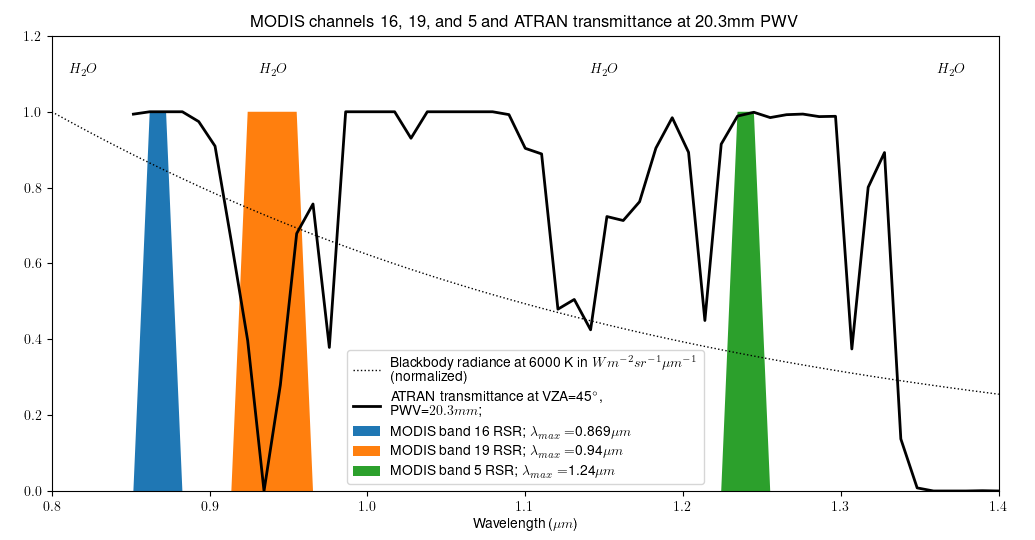
\includegraphics[width=.9\linewidth]{figures/atran_ref.png}
    \caption{Select MODIS channel spectral responses and ATRAN model transmittance at $20.3mm$ precipitable water vapor.}
    \label{p7_atran}
\end{figure}

In order to identify a pixel with high atmospheric transmittance I used a custom methodology inspired by the MOD03 water vapor product algorithm theoretical basis document, which points out that atmospheric transmittance is proportional to the ratio of TOA reflectance in an absorption channel to an expected clear-sky value estimated using nearby window channels.

According to (Richards, 2022) Figure 3.5, vegetation has a fairly linear spectral response function between the 2 window channels $\lambda_{w1}=.866\mu m$ and $\lambda_{w2}=1.242\mu m$. Thus, the TOA observed reflectance at these wavelengths describes a linear equation that can be used to estimate the clear-sky reflectance $R$ at an intermediate wavelength $\lambda' \in (\lambda_{w1}, \lambda_{w2})$ such that...

\begin{equation}\label{q7_ref_gain}
    R(\lambda') \approx \frac{R(\lambda_{w2})-R(\lambda_{w1})}{\lambda_{w2} - \lambda_{w1}} \times (\lambda'-\lambda_{w1}) + R(\lambda_{w1}) = g \times \Delta\lambda + R(\lambda_{w1})
\end{equation}

\begin{equation}\label{q7_gain_func}
    f(g) = \left( g \times (\lambda_{w2}-\lambda_{w1}) + R(\lambda_{w1})-R(\lambda_{w2}) \right)^2
\end{equation}

The intermediate wavelength $\lambda'=0.936\mu m$ (MODIS channel 19) is subject to absorption by atmospheric water vapor as shown in Figure \ref{p7_atran}. Therefore the atmospheric transmittance is proportional to the ratio of the water-attenuated reflectance in channel 19 to the expected clear-sky reflectance given observed vegetation reflectance in the surrounding window channels. This relationship is demonstrated in Figure \ref{p7_ref_graph}

In my case, coefficient $g$ in Equation \ref{q7_ref_gain} (the "gain" of the spectral response curve) is an unknown that only applies to the vegetation surface type. We can rearrange and square the equation to form a function $f(g)$ (Equation \ref{q7_gain_func}) that minimizes when the slope $g$ is close to the observed spectral response between the two window channels, which is useful for choosing the parameter. Ultimately, my selection procedure for a clear pixel consists of the following steps...

\clearpage

\begin{figure}[h!]
    \centering
        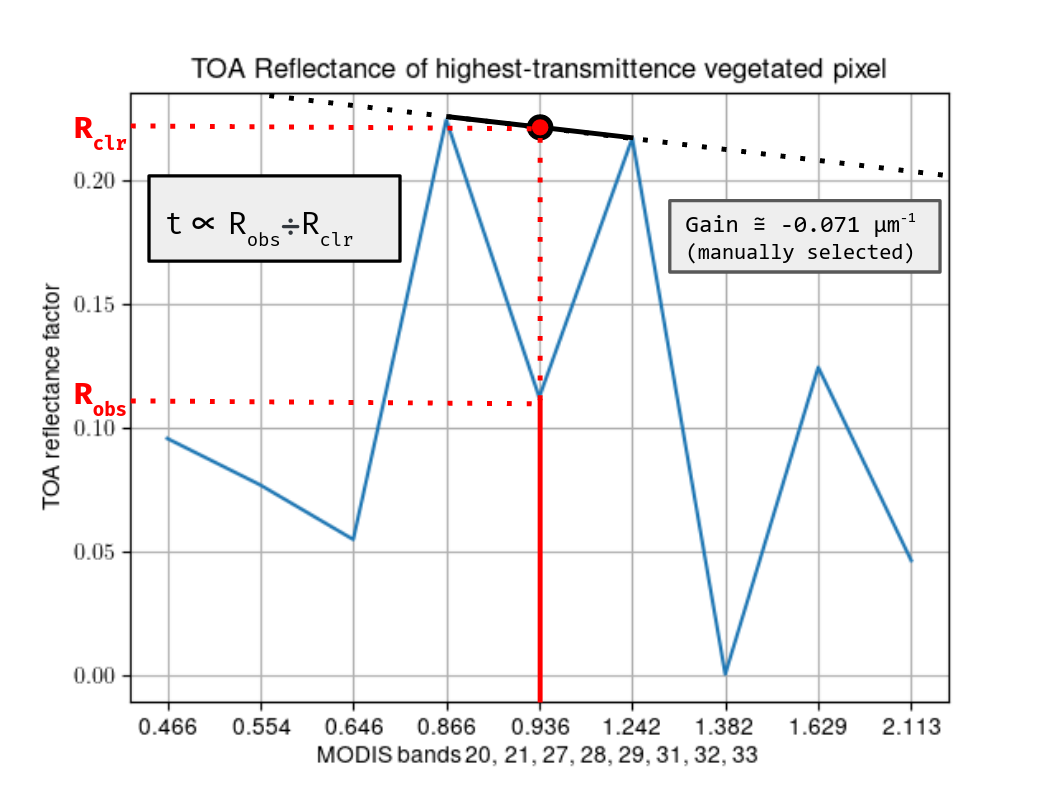
\includegraphics[width=.8\linewidth]{figures/trans_ref_annotated.png}

    \caption{Observed reflectances at clearest identified pixel, and annotations showing how atmospheric transmittance is estimated with my method. The $-0.071\mu m^{-1}$ slope was chosen manually to best match the spectral response of all vegetation in the image between the two window channels.}
    \label{p7_ref_graph}
\end{figure}

\noindent
\textbf{Clear-pixel identification:}
\begin{enumerate}
    \item{\textbf{Mask clouds} using Saunders \& Kriebel method with custom parameters.}
    \item{\textbf{Mask unvegetated surfaces} using a user-selected lower bound on NDVI.}
    \item{\textbf{Mask reflective surfaces} using a user-selected lower bound on total visible reflectance. This reflectance is the euclidean magnitude of the red, green, and blue channel reflectances, and is effective at masking pixels ``washed-out`` by aerosols and thin clouds.}
    \item{\textbf{Choose spectral response gain} by asking the user to manually choose a value that minimizes Equation \ref{q7_gain_func} over the surfaces not masked by steps 1-3.}
    \item{\textbf{Select pixel that maximizes transmittance}. This is the pixel that maximizes the ratio of clear-sky to observed reflectance in the absorption channel using the user-selected gain parameter.}
\end{enumerate}

All the custom parameters are selected using a GUI tool I developed that enables the user to choose a value with a slider and a live-rendered image. A demonstration of this process is available on my github and in the shared files.

\clearpage

\begin{figure}[h!]
    \centering
    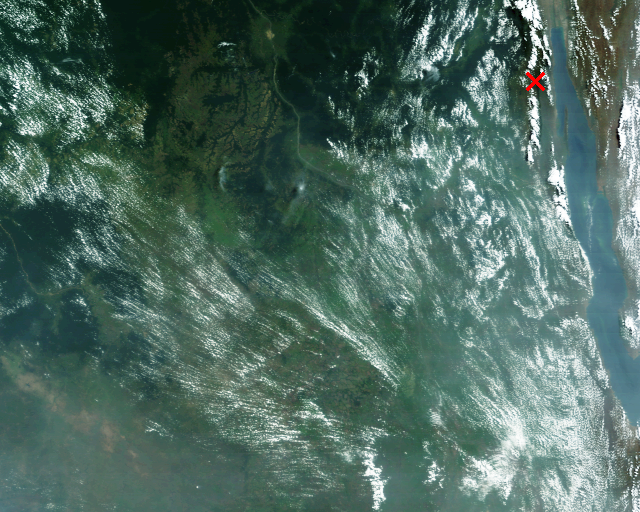
\includegraphics[width=.7\textwidth]{figures/trans_marker.png}

    \vspace{.8em}

    \begin{tabular}{R | C C C C C C C C C}
        \lambda\,\,(\mu m) & 0.466 & 0.554 & 0.646 & 0.866 & 0.936 & 1.242 & 1.382 & 1.629 & 2.113 \\
        \hline
        \rho & .096 & 0.077 & 0.055 & 0.224 & 0.112 & 0.217 & 0.000 & 0.124 & 0.046 \\
    \end{tabular}

    \vspace{.5em}

    \begin{tabular}{R | C C C C C C C C C}
        \lambda\,\,(\mu m) & 3.787 & 3.992 & 6.767 & 7.338 & 8.527 & 11.004 & 12.019 & 13.365 \\
        \hline
        T_B\,\,(K) & 293.412 & 292.984 & 249.635 & 263.240 & 288.103 & 289.963 & 289.410 & 268.218 \\
    \end{tabular}
    \caption{Clear pixel location, and TOA reflectances and brightness temperatures. Selected with a vegetation spectral response slope of $-0.07059 \mu m^{-1}$.}
    \label{p7_tables}
\end{figure}

The pixel my procedure ultimately selected is in a visibly clear region on the bank of Lake Tanganyika. The pixel's location and observed reflectances and brightness temperatures are shown in Figure \ref{p7_tables}, and the reflective and thermal spectral response curves of the pixel are shown by Figures \ref{p7_ref_graph} and \ref{p7_temp_graph}, respectively.

As a baseline for modeling transmittance in terms of column vapor, I scaled the atmospheric transmittance data used in Figure \ref{p7_atran} pointwise by the MODIS relative spectral response (RSR) function for band 19, which I retrieved from the EUMETSAT website. I generated the transmittance data using the NASA ATRAN model in a subtropical environment with solar zenith angle $45^\circ$ and precipitable water vapor of $20.3mm$. Since both the ATRAN and RSR data are normalized on $[0,1]$, the total transmittance is the average of the pointwise product on the valid range, which I determined to be $0.2477$ at $PWV=20.3mm$. With the weak assumption that transmittance $t$ varies linearly with precipitable water vapor $p$ and that water vapor is the exclusive cause of absorption, this model suggests that in range of MODIS band 19 ($1.242\mu m$) transmission decreases by $3.71\%$ per $mm$ PWV, as shown in Equation \ref{p7_modeltrans}.

\begin{equation}\label{p7_modeltrans}
    \frac{dt}{dp} = \frac{.2477-1}{20.3mm-0} = -0.0371\,\,mm^{-1}
\end{equation}

\clearpage

We can now estimate the observed transmittance in range of MODIS channel 19 using Equation \ref{q7_ref_gain} with gain $g=-0.071\mu m^{-1}$, wavelength offset $\Delta \lambda = \lambda'-\lambda_{w1} = .07\mu m$, and bands 16 and 19 reflectances $R_{16} = .224$ and $R_{19}=.112$.

\begin{equation}\label{p7_obsrans}
    t = \frac{R_{obs}}{R_{clr}} = \frac{R_{19}}{g\Delta\lambda + R_{16}} = \frac{.112}{.219} = .5112
\end{equation}

\begin{equation}\label{p7_pwv}
    p = \frac{.5112-1}{-0.0371mm^{-1}} = 13.175mm
\end{equation}

\noindent
Then with Equation \ref{p7_modeltrans}, the total precipitable water vapor in the column is $13.175$mm as shown in Equation \ref{p7_pwv}. This suggests a fairly dry atmosphere at the pixel location. This value could be used to initialize models or perform atmospheric correction for specific bands using lookup tables.

\begin{equation}\label{p7_atmocor}
    R_{TOA} = \frac{(L_{obs} - L_p)\pi\,t(\phi)}{S_{\Delta\lambda}\cos(\theta)t(\theta) + I_{sky}}
\end{equation}

The $.640\mu m$ channel is in a region with little atmospheric attenuation, so the main factors influencing the difference between surface and TOA reflectance are the sky irradiance $I_{sky}$ and path radiance $L_p$ in Equation \ref{p7_atmocor}. The solar and viewing zenith angles are $\theta = 24.58^\circ$ and $\phi = 35.84^\circ$ respectively, and the TOA available solar irradiance is approximately $1.52 W\,m^{-2}nm^{-1}$, or $76W\,m^{-2}$ on the MODIS band 16 range ($.620-670\mu m$). Finally the observed TOA radiance is $25.152 W\,m^{-2}\mu m^{-1}sr^{-1}$. Using conservative sky and path irradiance values of 10 $W\,m^{-2}$ and .5 $W\,m^{-2}sr^{-1}$, the theoretical reflectance with no atmospheric attenuation is $R_{TOA} = 0.312$. I'm not sure why the observed reflectance of $0.055$ is much lower than the theoretical value.

\begin{figure}[h!]
    \centering
        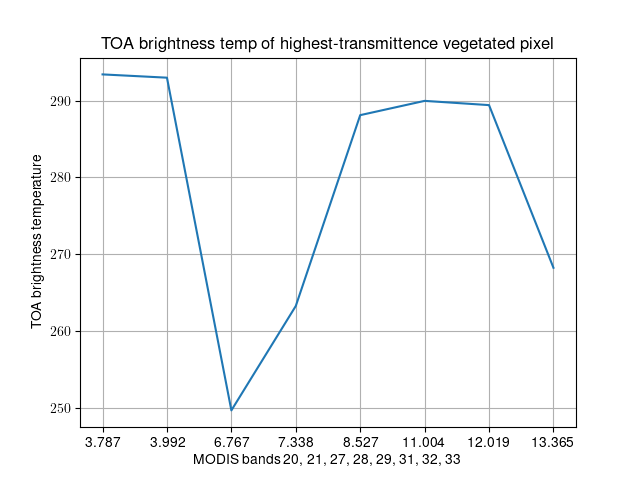
\includegraphics[width=.8\linewidth]{figures/trans_temp.png}

    \caption{Observed brightness temperature at clearest identified pixel.}
    \label{p7_temp_graph}
\end{figure}

Figure \ref{p7_temp_graph} displays the distribution of observed brightness temperatures for the same clear pixel. Since the identified pixel has a low water vapor content, atmospheric attenuation in the $11\mu m$ window channel should be very low. This means the greatest factor causing the brightness temperature to differ from the actual land surface temperature is the emissivity of the observed surface.

\begin{equation}\label{planck}
        %B(\lambda, T) = \frac{2hc^2}{\lambda^5 \left(\exp\left(\frac{hc}{\lambda k T}\right)-1\right)}
        T(\lambda, L_\lambda) = \frac{hc}{k \lambda \ln\left(\frac{2\epsilon hc^2}{\lambda^5 L_\lambda} + 1\right)}
\end{equation}

Since the pixel was specifically selected to be vegetated, I assume a typical vegetation emssivity of $\epsilon = .93$. The original observed radiance at $11\mu m$ is $8.21598 W\,m^{-2}\mu m^{-1} sr^{-1}$. Applying the inverse planck function (Equation \ref{planck}) with the radiance scaled by the surface emissivity, I determined that the approximate land surface temperature is $294.65K$, about $5K$ warmer than the observed brightness temperature.

\clearpage

\section{K-means classification}

\begin{figure}[h!]
    \centering
        \makebox[\textwidth]{
            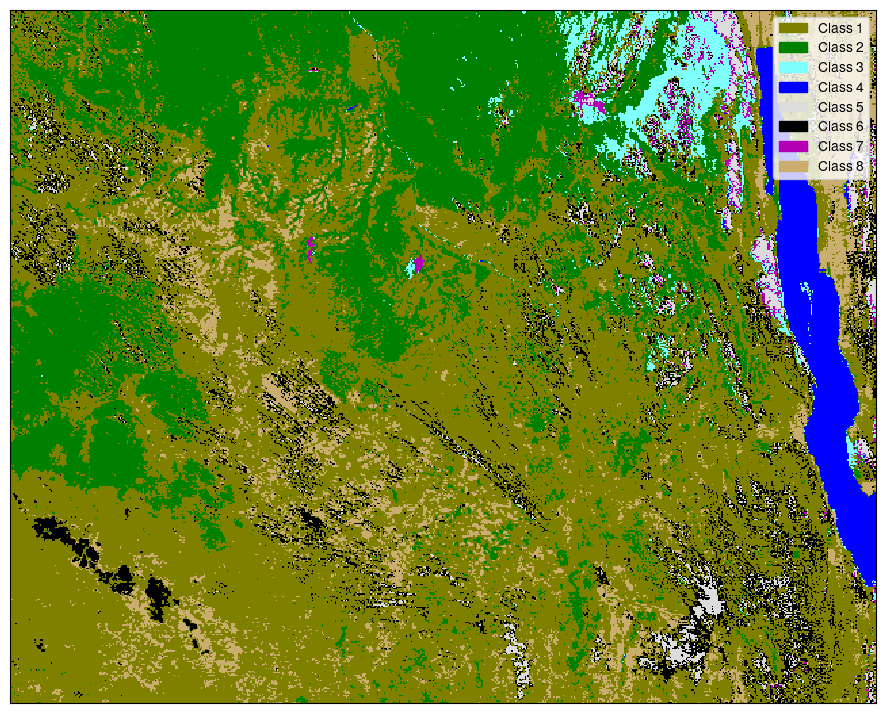
\includegraphics[width=.45\paperwidth]{figures/k_means_8c_all_2.png}

            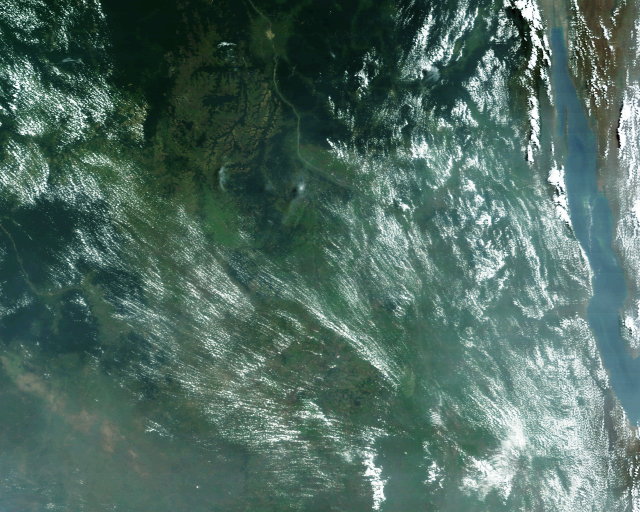
\includegraphics[width=.45\paperwidth]{figures/rgb_tc.png}
        }

    \caption{K-means classification results with 8 classes, and original truecolor RGB.}
    \label{p8_km}
\end{figure}

\begin{figure}[h!]
    \centering

    \begin{tabular}{c | c | c}
        Band & Wavelength range & Justification \\
        \hline
        1     & 620-670nm      & NDVI, general VIS reflectance \\
        16    & 862-877nm      & aerosol distinction, NDVI \\
        5     & 1230-1250nm    & optical depth \\
        26    & 1360-1390nm    & thin cirrus identification \\
        6     & 1628-1652nm    & cloud phase \\
        7     & 2106-2155nm    & cloud particle size \\
        21    & 3929-3989      & SWIR, fire identification and water \\
        29    & 8400-8700nm    & Infrared cloud phase, emissivity diff 11-8.5um \\
        31    & 10780-11280nm  & clean LWIR; cloud-top and land surface temp\\
    \end{tabular}
    \caption{Selected MODIS bands for k-means classification and justification}
    \label{p8_just}
\end{figure}

Figure \ref{p8_km} shows my migrating means classification results, which I performed using the MODIS channels outlined in Figure \ref{p8_just} with each array normalized to $[0,1]$. The classified array has high skill in distinguishing water and 3 distinct land surface types, as well as multiple cloud types, but struggles to separate low and optically-thin clouds from arid ground with an optically thick (smoky) atmosphere, as suggested by the ``Class 6'' patch at the lower left of the image.

\clearpage

\begin{figure}[h!]
    \centering
    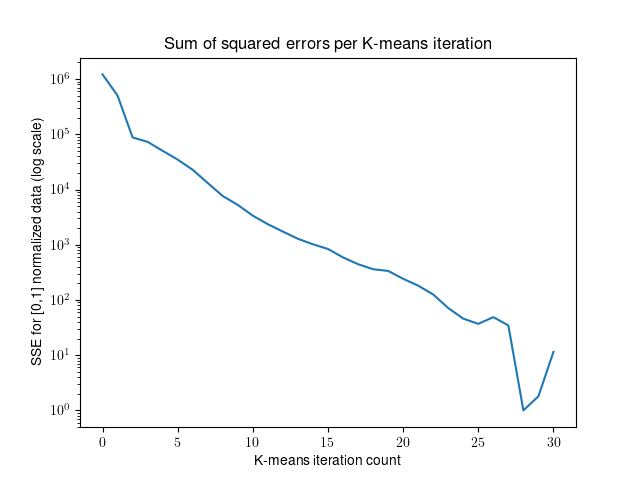
\includegraphics[width=.8\linewidth]{figures/k_means_sse_2.png}

    \begin{tabular}{c | c c c c c c c c }
        Class & KM1 & KM2 & KM3 & KM4 & KM5 & KM6 & KM7 & KM8 \\
        \hline
        water & 0 & 0 & 0 & 100 & 0 & 0 & 0 & 0 \\
        cirrus & 83 & 17 & 0 & 0 & 0 & 0 & 0 & 0 \\
        low cloud & 8 & 0 & 0 & 0 & 66 & 26 & 0 & 0 \\
        deep cloud & 0 & 0 & 3 & 0 & 84 & 0 & 13 & 0 \\
        rainforest & 0 & 100 & 0 & 0 & 0 & 0 & 0 & 0 \\
        savanna & 100 & 0 & 0 & 0 & 0 & 0 & 0 & 0 \\
        fire & 9 & 0 & 0 & 0 & 1 & 5 & 0 & 7 \\
    \end{tabular}
    \caption{Sum of squared errors and confusion matrix between sample classes and K-means clustering results. Note that all sample classes have 100 members except for the fire class, which has only 22. Rainforest, savanna, and water surface samples were entirely covered by corresponding k-means class, but there is increased variation in the cloud type results. This is partially due to the larger number of K-means classes than original classes, as the result appears to resolve mid-level clouds with $KM5$ separately from low clouds ($KM6$ and $KM4$). Although the cirrus samples I chose were evidently too optically thin for this method to realize them, other cirrus in the image appear to be effectively masked by $KM3$, and tall optically-thick clouds are represented by $KM7$.}
\end{figure}

\clearpage

\section{Extra figures}

\begin{figure}[h!]
    \centering
    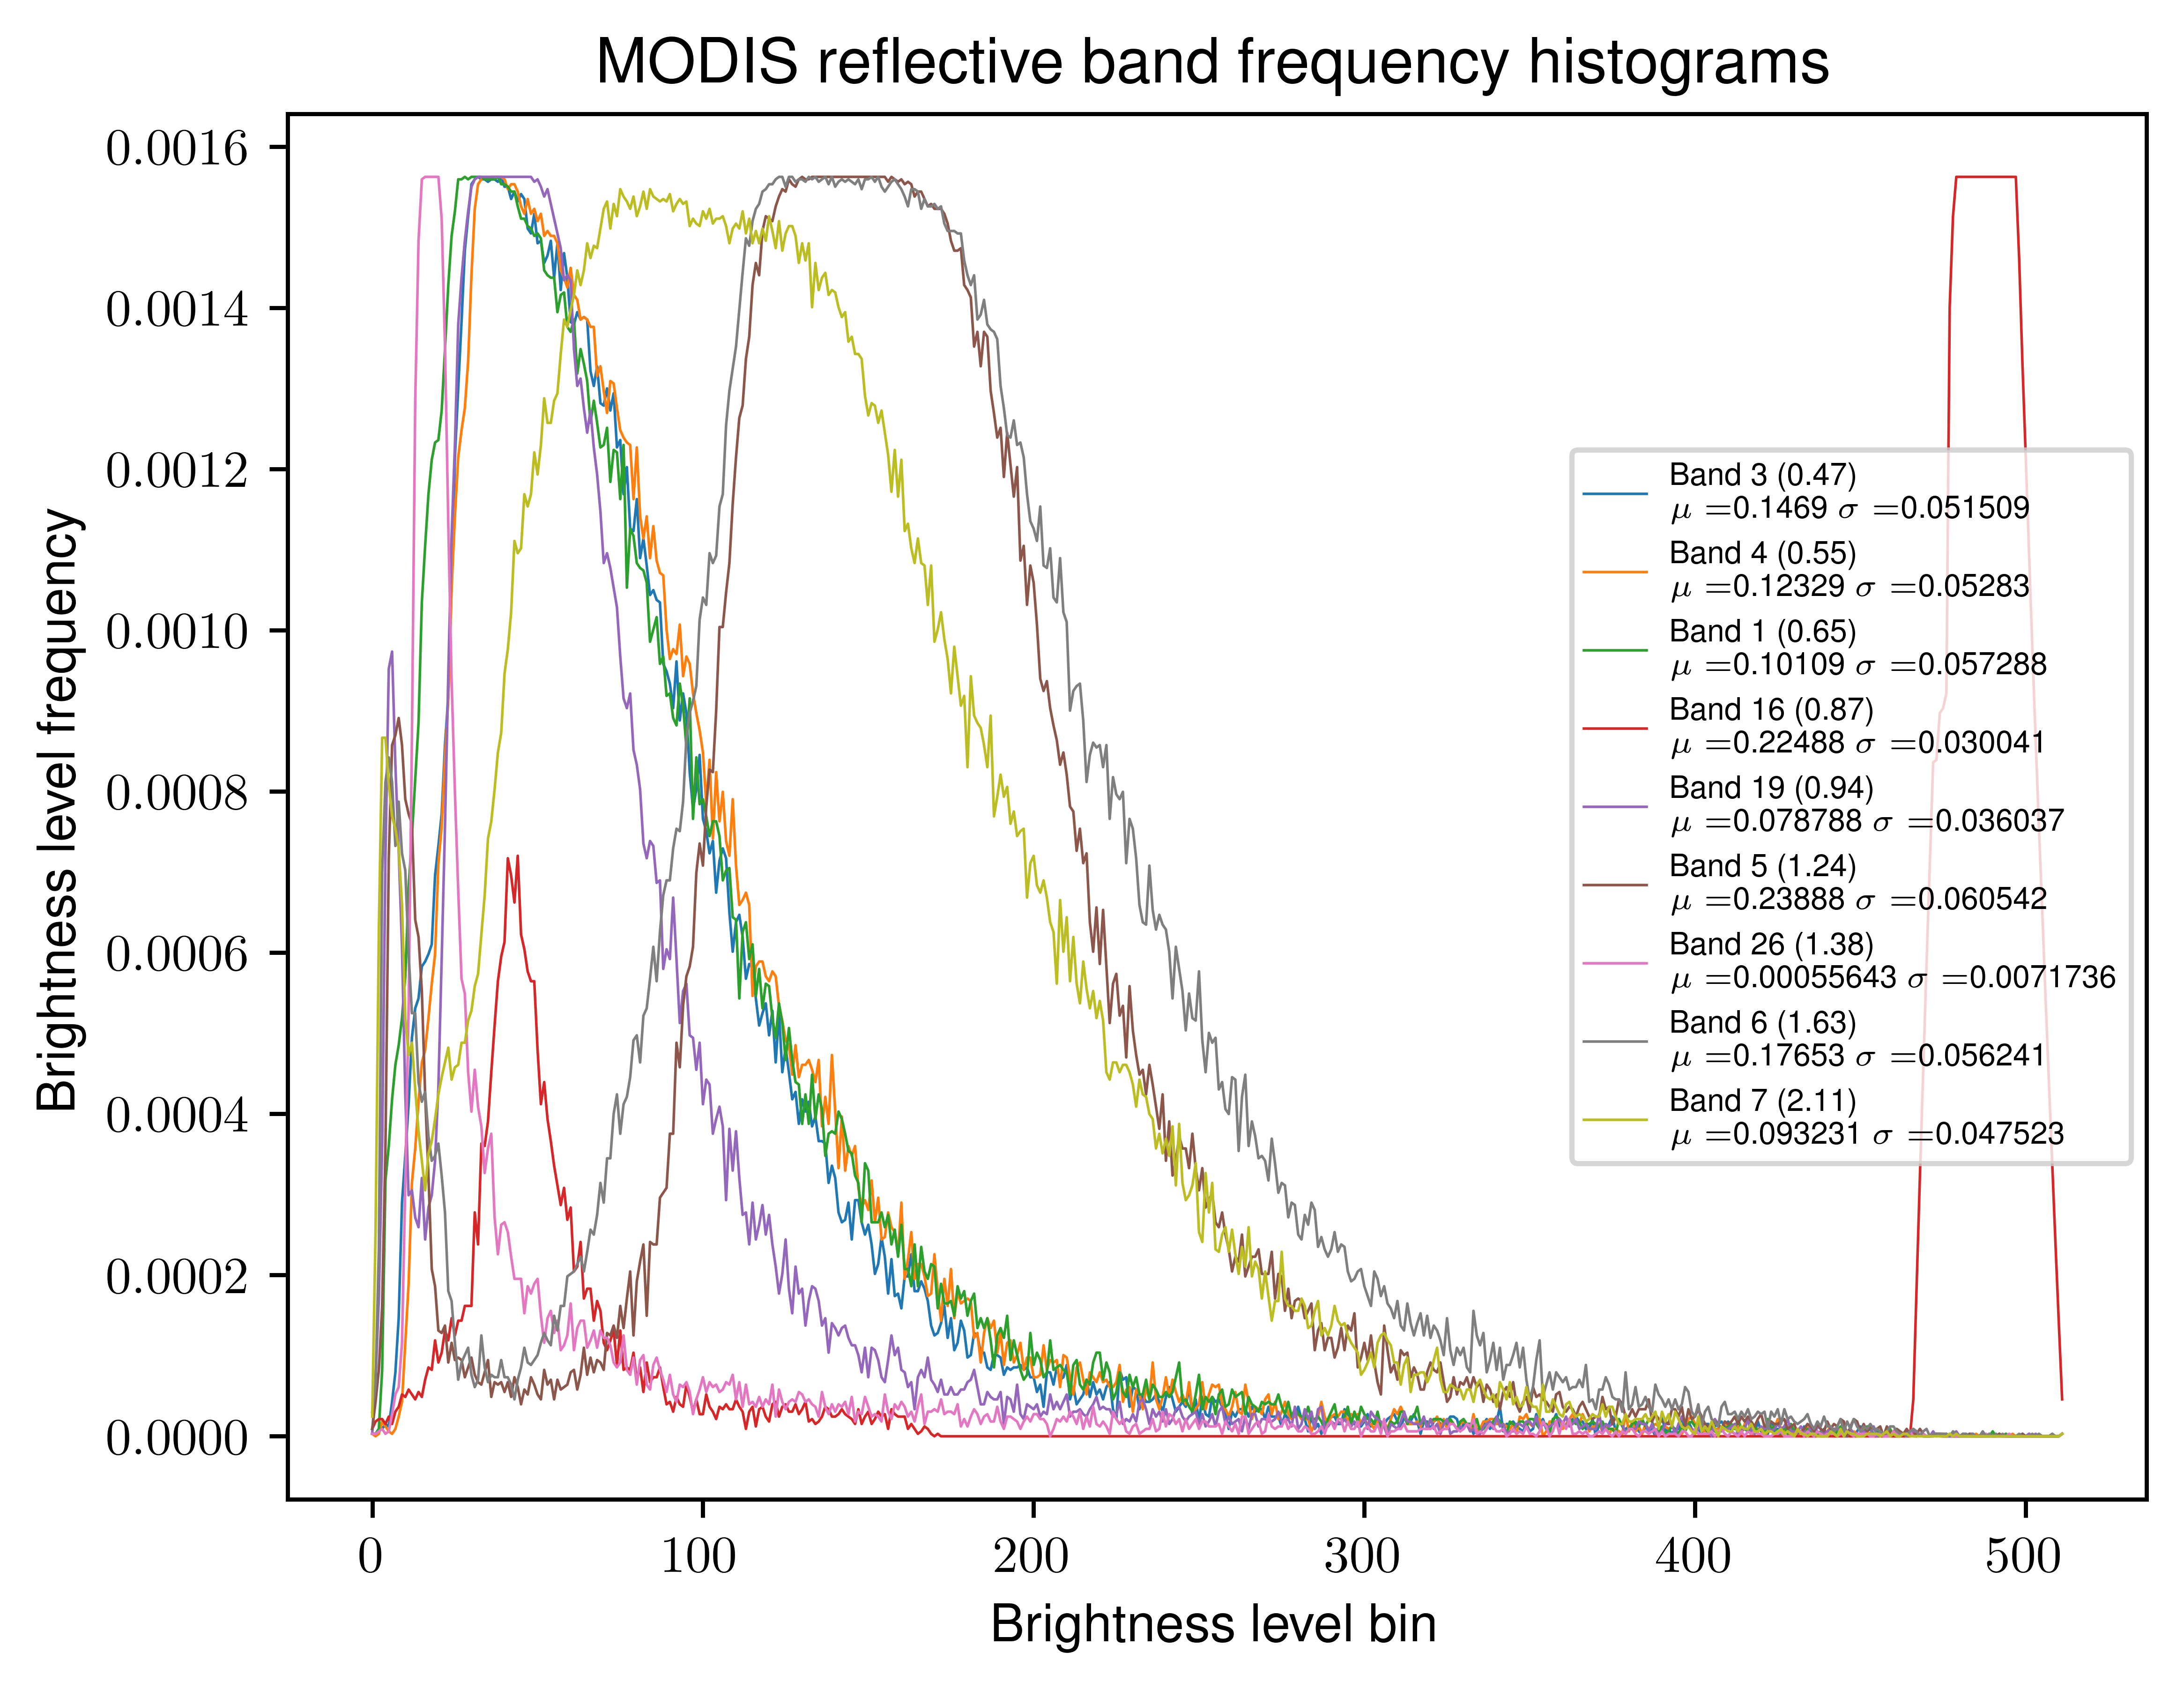
\includegraphics[width=.8\textwidth]{figures/hists_ref.png}
    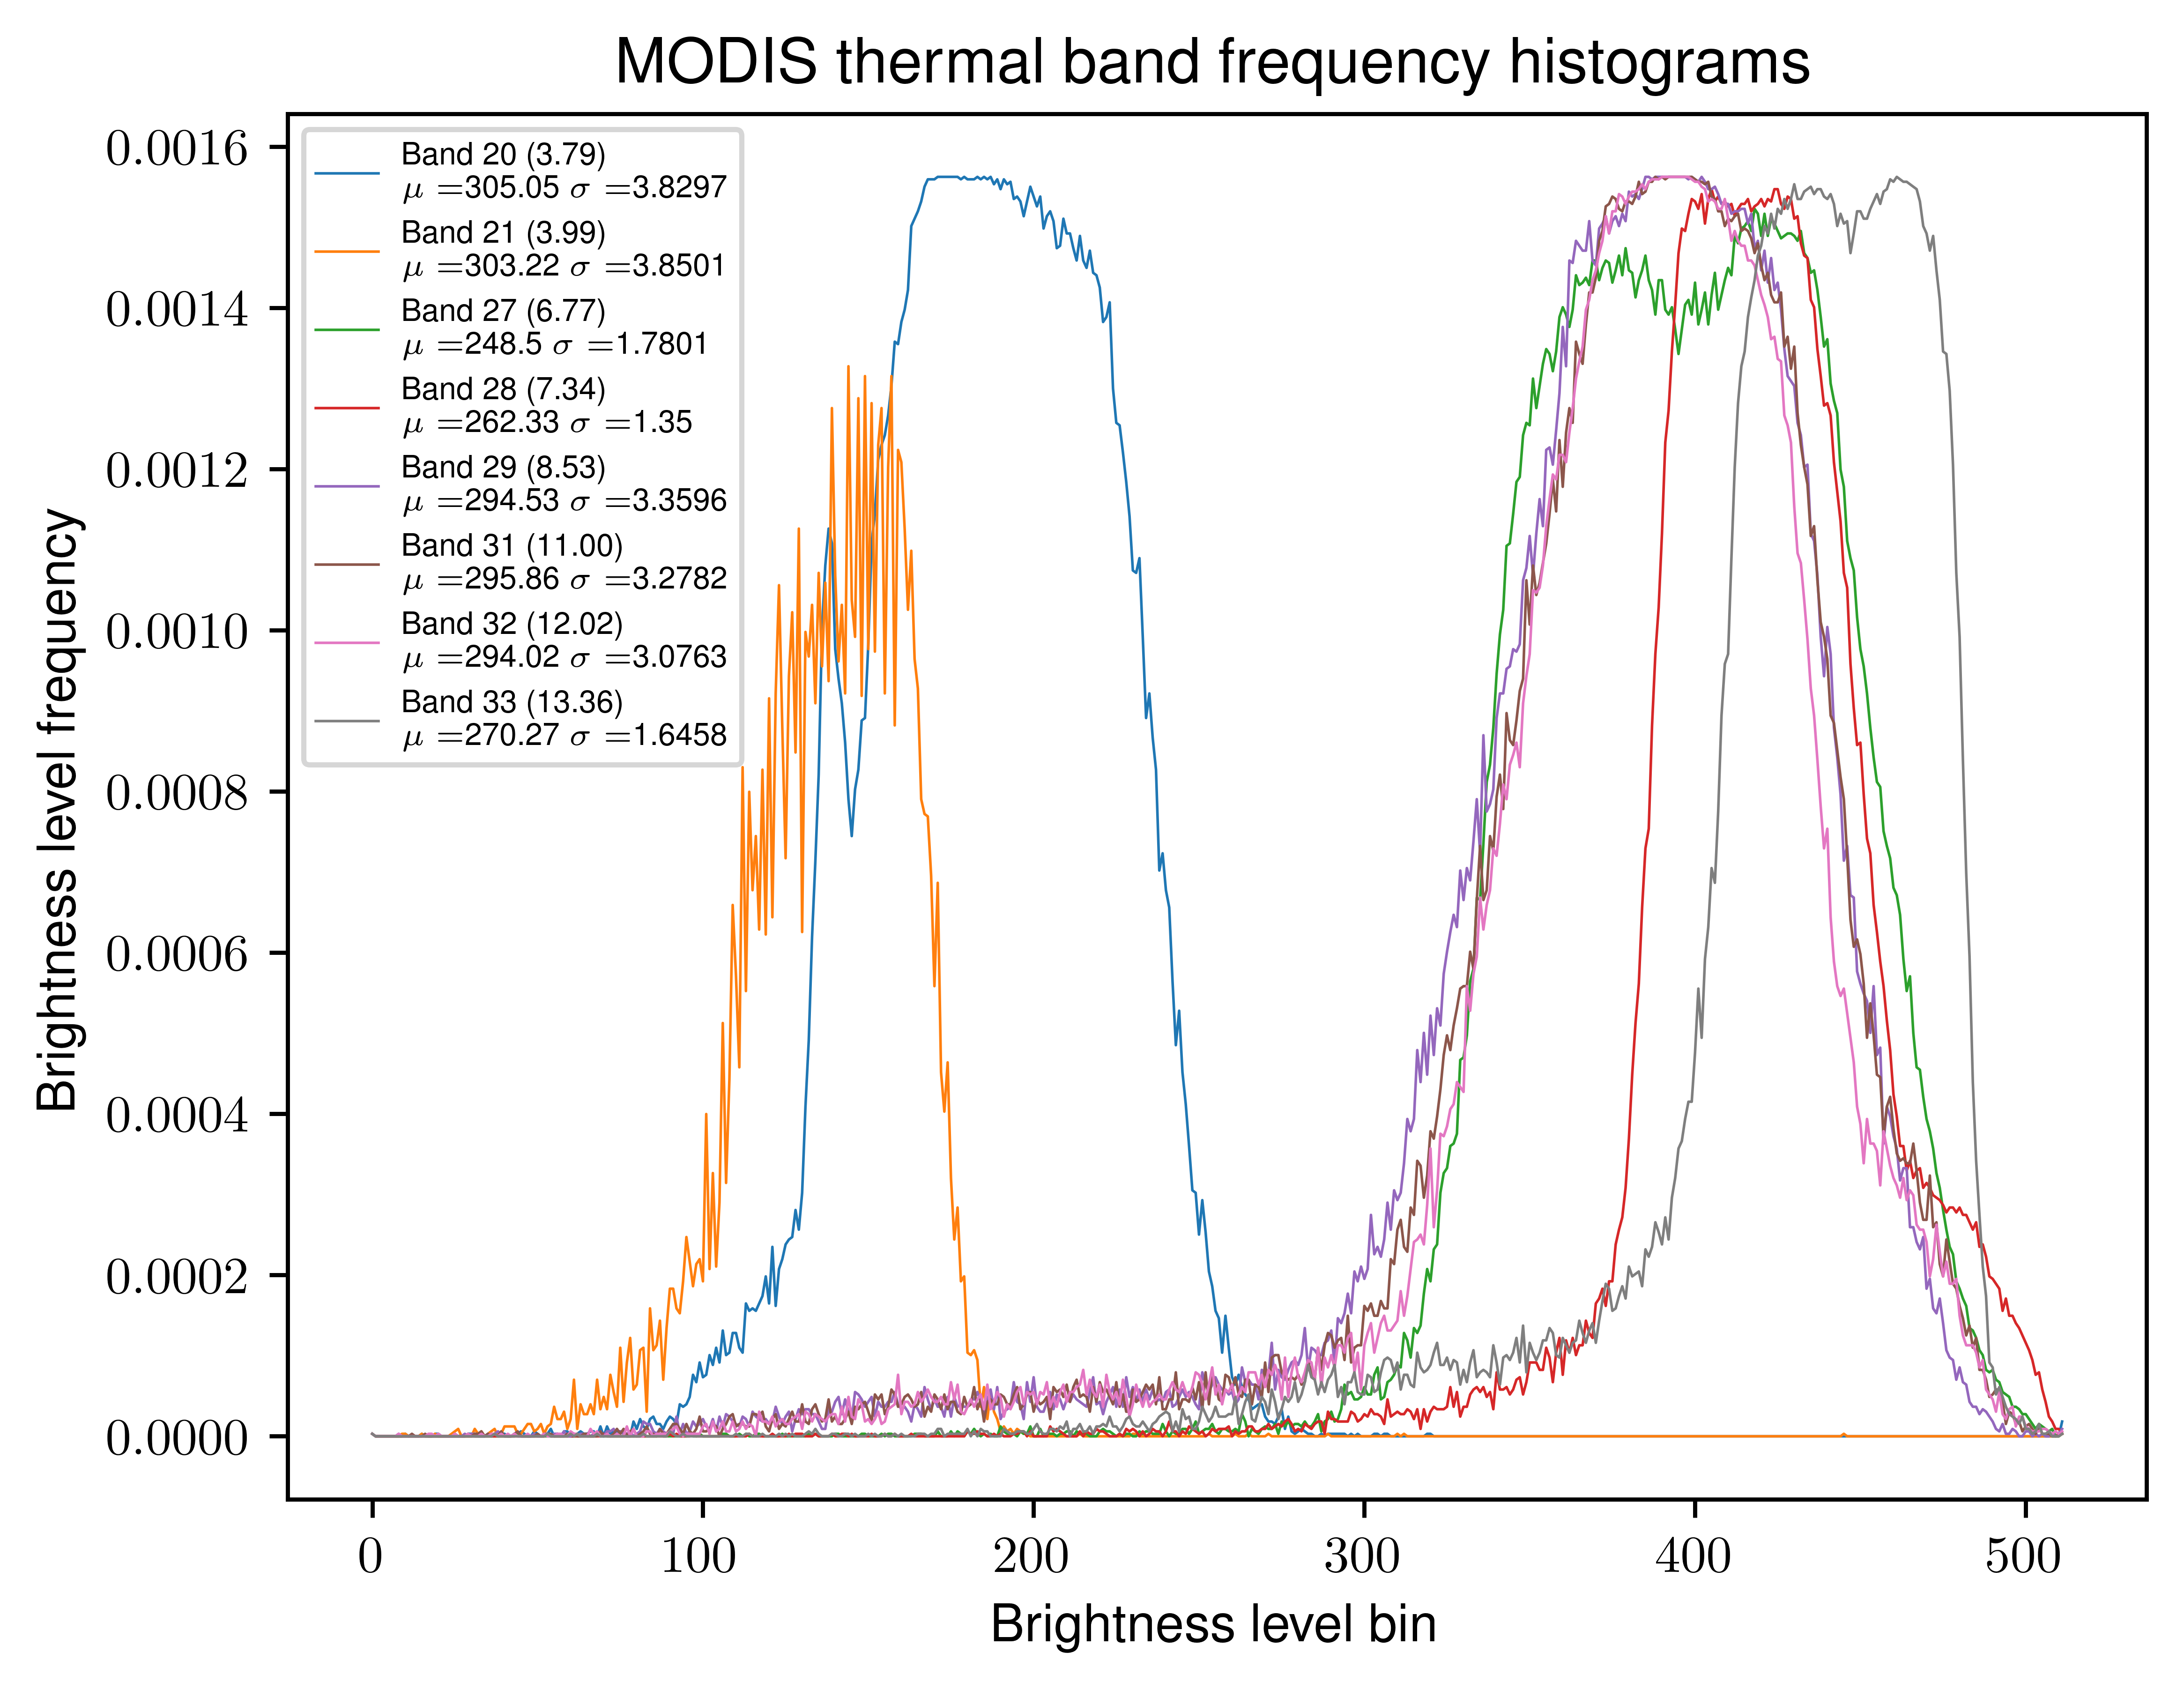
\includegraphics[width=.8\textwidth]{figures/hists_tb.png}
    \caption{MODIS band brightness histograms}
    \label{}
\end{figure}

\end{document}
